
Parámetros del test: 
Cantidad de iteraciones por filtro-version 20.
ALFA 150

\begin{figure}[h]
  \begin{center}
	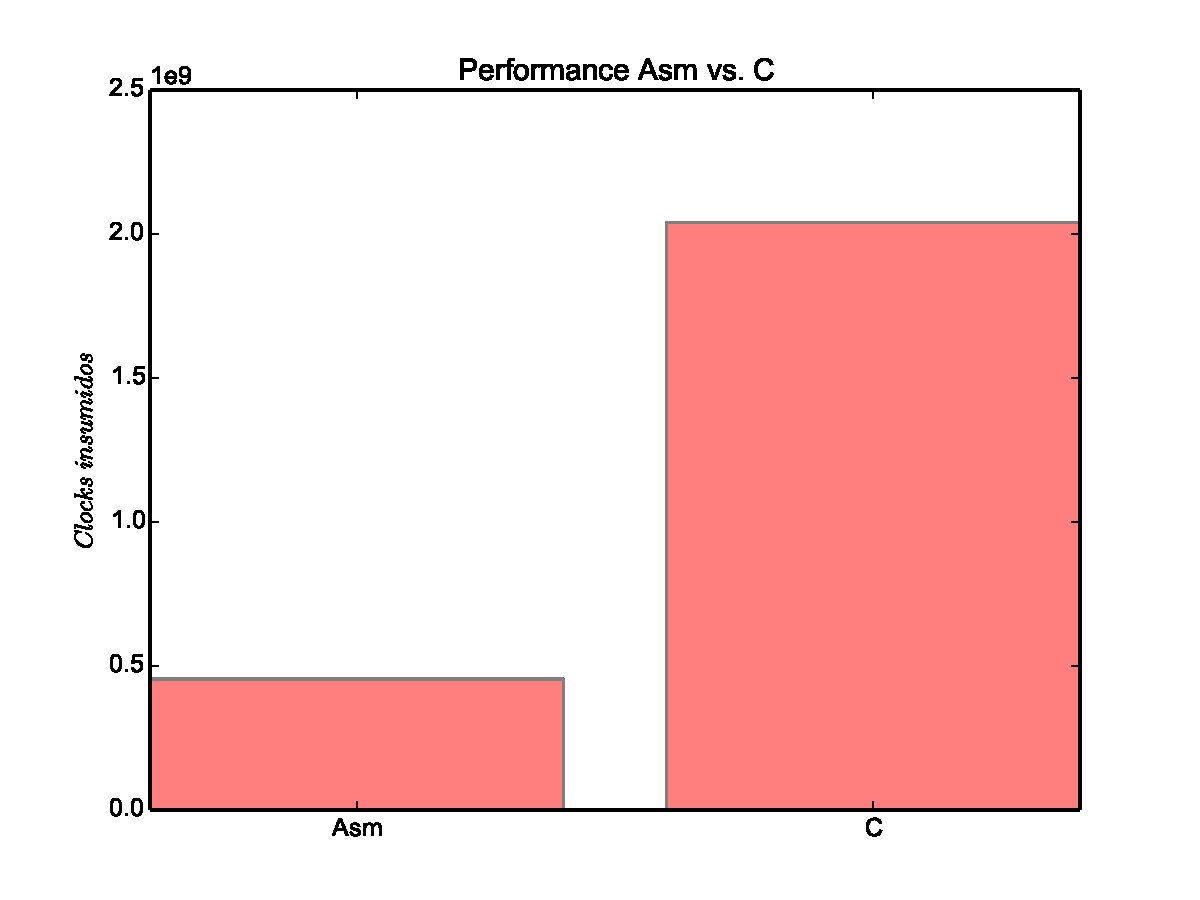
\includegraphics[scale=0.5]{ldrA.pdf}
	%\caption{La última de Star Wars}
  \end{center}
\end{figure}

\begin{figure}[h]
  \begin{center}
	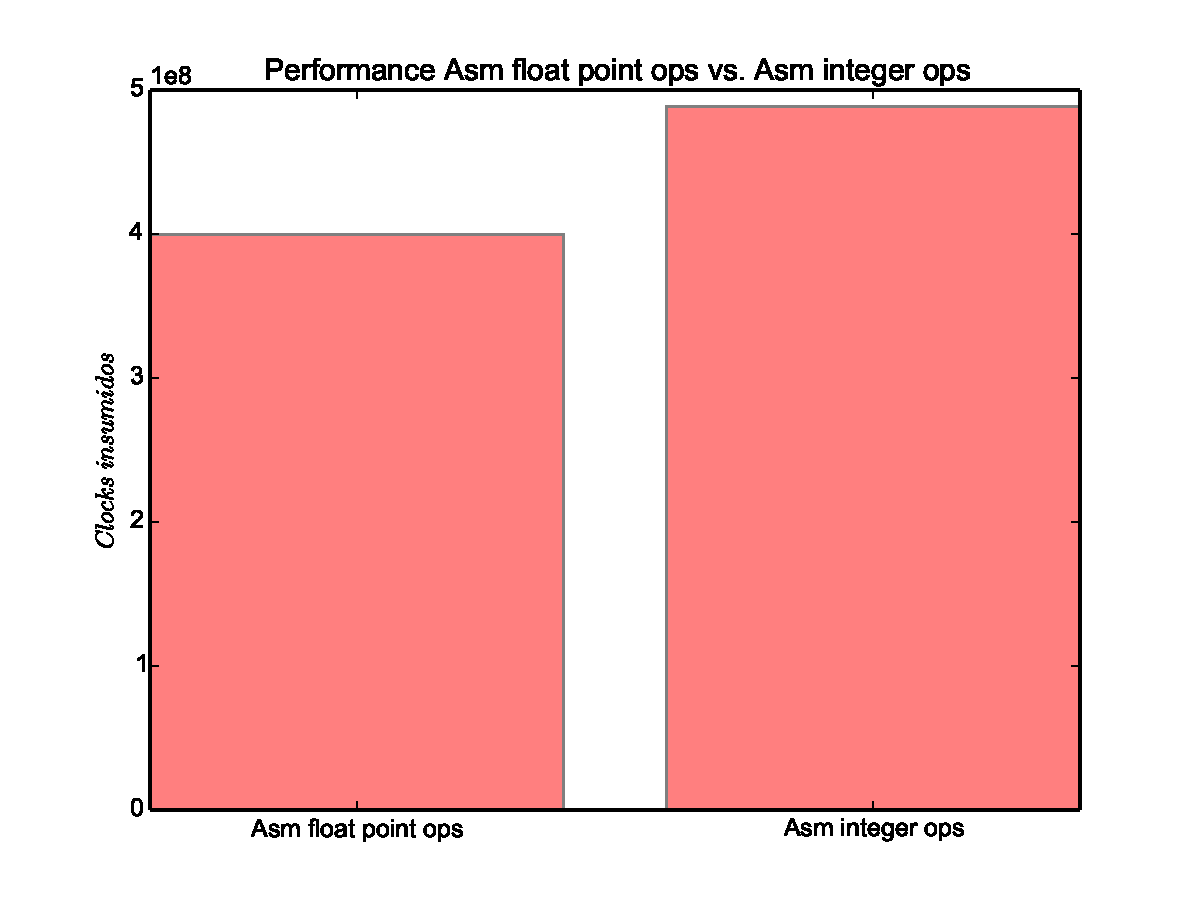
\includegraphics[scale=0.5]{ldrB.pdf}
	%\caption{La última de Star Wars}
  \end{center}
\end{figure}


$a)$ Gana $assembler$. Claramente los accesos no suponen un problema, dado que por principo de vecinidad espacial, en la cache al leer un pixel, se traera consigo varios contiguos. La diferencia radica en el procesamiento paralelo que SIMD nos permite.

$b)$ Gana con ops en punto flotante: Para este caso particular, al menos, el hecho de tener que dividir cada escalar por separado no supone una ventaja, todo lo contrario. Y al final es mas conveniente operar en punto flotante, dado que ya veniamos procesando en paralelo. Esto es particular a la implementacion y a los cambios requeridos. Muy probablemente si se hubiese llevado a cabo en sepia hubiese arrojado otros resultados, debido a que podriamos operar con enteros sin perder paralelismo.
